I dette afsnit definerer vi grænseværdien for en funktion stringent med den såkaldte $\varepsilon $-$\delta $-definition.
Vi arbejder dog kun med reele funktioner med delmængder af $\mathbb{R}$ som definitionsmængde. 

Vi undersøger så kontinuerte funktioner med lukkede intervaller som definitionsmængde, da disse funktioner har nogle specielle egenskaber, der ikke er gældende for alle kontinuerte funktioner.
Disse resultater benyttes senere til at bevise vigtige resultater for Riemann-integralet.

\subsection{Grænseværdier af reele funktioner af delmængder af $\mathbb{R}$}%
\label{sub:Grænseværdi}
\begin{definition}[label=def:grænseværdi]{Grænseværdi af funktion}{}
  Antag $X \subseteq \mathbb{R}$, $f:X \to \mathbb{R}$, og $p$ er et fortætningspunkt af $X$.
  Et tal $L$ kaldes for grænseværdien af $f$ i $p$ og vi skriver
  \[
  \lim_{x \to p} f(x)= L,
  \] 
  hvis der for alle $\varepsilon >0$ eksisterer et tal $\delta >0$ sådan at når $x \in X$ og $0<\abs{x-p} < \delta  $, så gælder $\abs{f(x)-L} <\varepsilon $.  
\end{definition}

\begin{figure}[H]
\begin{center}
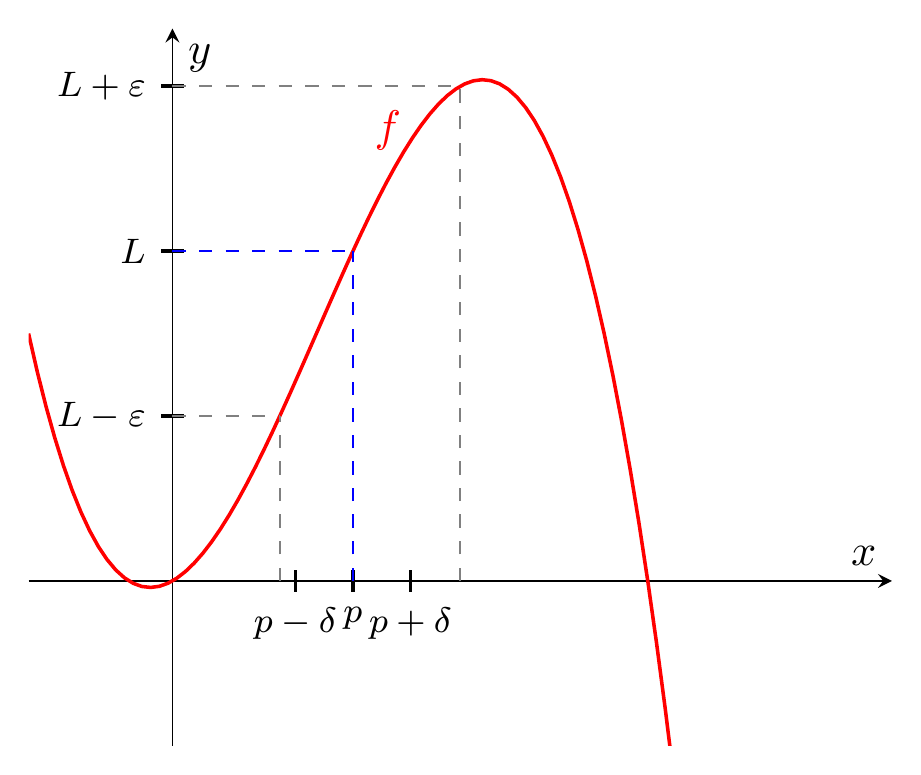
\begin{tikzpicture}[scale=1.6, transform shape]
\begin{axis}[xmin=-1, xmax=5, ymin=-2, ymax=6.7, axis lines=middle,
  xlabel=$x$,ylabel=$y$,
  xtick={0.8541,1.2541,1.6541},
  xticklabels={$p- \delta $, $p$, $p+\delta $},
  xticklabel style={anchor=north, font=\footnotesize},
  ytick={2,4,6},
  yticklabels={$L-\varepsilon $, $L$, $L+\varepsilon $},
  every major tick/.append style={thick, major tick length=5pt, black},
  yticklabel style={anchor=east, font=\footnotesize}
  ]
  \addplot[color=red, domain=-1:5, samples=100, thick]{-x^3 + 3*x^2+x} node[left, pos=0.15] {$f$};
  \draw[color=gray, dashed] (axis cs:0.7459,0) -- (axis cs:0.7459,2);
  \draw[color=gray, dashed] (axis cs:0,2) -- (axis cs:0.7459,2);
  \draw[color=gray, dashed] (axis cs:2,0) -- (axis cs:2,6);
  \draw[color=gray, dashed] (axis cs:0,6) -- (axis cs:2,6);
  \draw[color=blue, dashed] (axis cs:1.2541,0) -- (axis cs:1.2541,4);
  \draw[color=blue, dashed] (axis cs:0,4) -- (axis cs:1.2541,4);
\end{axis}
\end{tikzpicture}
\end{center}
\caption{$\varepsilon $-$\delta $-definition af funktionel grænseværdi}%
\label{fig:epsilondelta}
\end{figure}

Bemærk, at siden $p$ ikke behøver være i definitionsmængden $X$ (se eksempel \ref{exa:fortætningspunkter}), så kan grænseværdien for $f$ sagtens give mening i punkter, hvor selve $f$ ikke er defineret.

\begin{example}[label=exa:grænseværdi]{Grænseværdi i punkt, hvor funktion ikke er defineret}{}
 Lad funktionen $f:\{ x \in \mathbb{R}:x>0 \} \to \mathbb{R}$ være defineret ved
  \[
  f(x)= x^2.
  \] 
  Fra eksempel \ref{exa:fortætningspunkter} har vi, at $0$ er et fortætningspunkt af $\{ x \in \mathbb{R}:x>0 \} $. 
  Vores intuition fortæller os så, at
  \[
  \lim_{x \to 0} f(x)= 0.
  \] 
  Dette vil vi nu bevise stringent via definition \ref{def:grænseværdi}.

  For alle $\varepsilon >0$ vælger vi $\delta =\sqrt{\varepsilon } $. 
  Så har vi, at når $x \in \{ x \in \mathbb{R}:x>0 \} $ og $0<\abs{x-0} =\abs{x} <\delta $, så gælder
  \[
    \abs{f(x)-0} =\abs{x^2}=\abs{x}^2<\delta ^2=\varepsilon.
  \] 
  Altså har vi vist, at $\lim\limits_{x \to 0}f(x)=0$.
\end{example}

Det næste eksempel viser, at selv hvis et punkt $p$ tilhører definitionsmængden af en funktion $f$, så kan vi trods intuitionen godt have $\lim\limits_{x \to p} f(x) \neq f(p)$.

\begin{example}[label=exa:grænseværdi2]{Grænseværdi af funktion i punkt ulig funktionsværdien}{}
  
\end{example}

\subsection{Kontinuerte funktioner på intervaller}%
\label{sub:Kontinuert}


\begin{definition}[label=def:kontinuert]{Kontinuert}{}
 Antag $X \subseteq \mathbb{R}$, $f:X \to \mathbb{R}$ og $p \in X$.

  Så er $f$ kontinuert i $p$, hvis der for alle $\varepsilon >0$ eksisterer $\delta >0$ sådan at når $x \in X$ og $\abs{x-p} < \delta  $, så gælder $\abs{f(x)-f(p)}<\varepsilon $. 

  Hvis $f$ er kontinuert i alle punkter i $X$, så siger vi, at $f$ er kontinuert på $X$. 
\end{definition}

Ved første øjekast ligner dette definitionen af grænseværdier af funktioner til forveksling.
Den største forskel ligger i, at vi her kræver, at $f$ skal være defineret i $p$. 
Tilvarende skal vi i \cref{fig:epsilondelta} blot skrive $f(p)$ i stedet for $L$, for at figuren illustrerer definitionen på kontinuitet. 

Sammenligner vi med definition \ref{def:grænseværdi}, ser vi, at hvis vi også antager, at $p$ er et fortætningspunkt af $X$, så er $f$ kontinuert i $p$ præcis når
\[
\lim_{x \to p} f(x) =f(p).\footnote{Kontinuitet defineres sådan i f.eks. \cite{Brydensholt2018}, s. 34. Bemærk, at grænseværdien $\lim\limits_{x \to p} f(x)$ ikke giver nogen mening, hvis $p$ er et isoleret punkt af $X$.}
\] 
Derudover medfører vores definition, at en funktion er kontinuert i alle isolerede punkter af dens definitionsmængde. 
\begin{example}[label=exa:kontinuert_i_isoleret]{Funktioner er kontinuerte i isolerede punkter af dens definitionsmængde}{}
 Antag $X \subseteq \mathbb{R}$, $f:X \to \mathbb{R}$, og $p$ er et isoleret punkt af $X$. 

  Så er $p$ ikke et fortætningspunkt af $X$, hvilket vil sige, at der eksisterer en omegn $N_r(p)$ sådan at ${N_r(p) \cap X=\{ p \}  }$.
  For alle $\varepsilon >0$ kan vi så vælge $\delta =r$. 
  Så har vi, at når $x \in X$ og $\abs{x-p} <\delta $, så gælder
  \[
  \abs{f(x)-f(p)}=0<\epsilon.
  \] 
  Altså er $f$ kontinuert i $p$. 
\end{example}


\begin{definition}[label=def:begrænset_funktion]{Begrænset funktion}{}
  Antag $X \in \mathbb{R}$.
  Så er en funktion $f:X \to \mathbb{R}$ begrænset, hvis der eksisterer $M \in \mathbb{R}$ sådan at $\abs{f(x)}\leq M$ for alle $x \in X$. 
\end{definition}

Det næste resultat viser, at en kontinuert funktion på et lukket interval er begrænset.

\begin{theorem}[label=theo:kontinuert_begrænset]{Kontinuert funktion på lukket interval er begrænset}{}
  Hvis en funktion $f:[a;b] \to \mathbb{R}$ er kontinuert, så er den begrænset.  
\end{theorem}
\begin{proof} 
  
\end{proof}

\begin{theorem}[label=theo:kontinuert_maks]{Kontinuert funktion på luklet interval har maksimum og minimum}{}
  Antag $f:[a;b] \to \mathbb{R}$ er kontinuert, og lad $\Vm(f)=\{ f(x):x \in [a;b] \} $.
  Så eksisterer $p,\,q \in [a;b]$ sådan at $f(p)=\sup \Vm(f)$ og $f(q)=\inf \Vm(f)$.
\end{theorem}
\begin{proof} 
  
\end{proof}


\begin{definition}[label=def:uniform_kontinuert]{Uniform kontinuert}{}
  Antag $X \subseteq \mathbb{R}$ og $f:X \to \mathbb{R}$. 
  Så er $f$ uniform kontinuert på $X$ hvis der for alle $\varepsilon >0$ eksisterer $\delta >0$ sådan at der for alle $p,\,q \in X$ gælder
  \[
  \abs{p-q} < \delta \implies \abs{f(p)-f(q)}<\varepsilon .  
  \] 
\end{definition}

